% file: 3-6-graph-decomposition/bicomp-cutnode-theorem.tex

\documentclass[tikz]{standalone}
\usetikzlibrary{positioning, shapes, decorations.pathmorphing}

\begin{document}
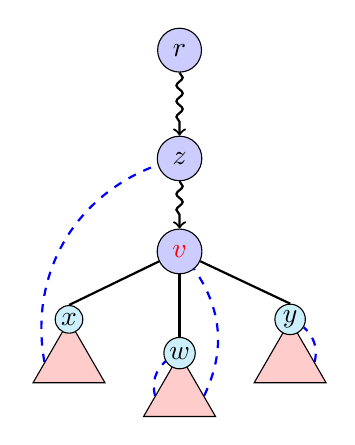
\begin{tikzpicture}[normal/.style = {circle, minimum size = 12pt, draw, fill = blue!20},
    smallv/.style = {circle, draw, inner sep = 1pt, fill = cyan!20},
    subtree/.style = {regular polygon, regular polygon sides = 3, minimum size = 30pt, draw, fill = red!20},
    every edge/.style = {draw, thick},
    sedge/.style = {->, decorate, decoration = {snake, amplitude =.4mm, segment length = 2mm, post length = 1mm}},
    bedge/.style = {dashed, blue}] 
  \node (1) [normal] {$r$};
  \node (2) [normal, below = 0.80cm of 1] {$z$};
  \node (v) [normal, below = 0.60cm of 2] {\textcolor{red}{$v$}};

  \node (m) [subtree, below = of v] {};
  \node (w) [smallv, at = (m.north)] {$w$};

  \node (l) [subtree, below left = of v] {};
  \node (x) [smallv, at = (l.north)] {$x$};

  \node (r) [subtree, below right = of v] {};
  \node (y) [smallv, at = (r.north)] {$y$};

  \path (1) edge[sedge] (2)
	(2) edge[sedge] (v)
	(v) edge (w)
	    edge (x.north)
	    edge (y.north)
	(l.west) edge[bedge, bend left = 40] (2)
	(m.east) edge[bedge, bend right] (v)
	(m.west) edge[bedge, bend left] (w)
	(r.east) edge[bedge, bend right] (y);
\end{tikzpicture}
\end{document}
